\documentclass[12pt]{article}
\usepackage{design_ASC}
\usepackage[T2A]{fontenc}
\usepackage[utf8]{inputenc}
\usepackage[russian]{babel}
\usepackage{hyphenat}
\hyphenation{ма-те-ма-ти-ка вос-ста-нав-ли-вать}

\setlength\parindent{0pt}

\title{Типовой расчет по математике\\Интегрирование функции одной переменной\\3 модуль}

\author{ФИО\\
Студент группы P3113\\
\textsc{Вариант №}}

\begin{document}
\setlength{\droptitle}{-5em}    

\maketitle

\subsection*{Задание 1. Проинтегрируйте методом внесения под знак дифференциала.}

$=$\vspace{2.5mm}

Ответ: $ $

\subsection*{Задание 2. Найдите интеграл от тригонометрической функции.}

$=$\vspace{2.5mm}

Ответ: $ $

\subsection*{Задание 3. Найдите интеграл.}

$=$\vspace{2.5mm}

/ $ $ \\
$ $ /

$=$\vspace{2.5mm}

Ответ: $ $

\subsection*{Задание 4. Найдите интеграл от дробно-рациональной функции.}

$=$\vspace{2.5mm}

$
\begin{cases}
A=\\
A+B=\\
A+B+C=\\
A+B+C+D=
\end{cases} \begin{cases}
A=\\
B=\\
C=\\
D=
\end{cases}\Rightarrow\vspace{2.5mm} \\
\Rightarrow $\vspace{2.5mm}

Ответ: $ $

\subsection*{Задание 5. Найдите интеграл от иррациональной функции.}

$=$\vspace{2.5mm}

/ Замена: $t=$ /\vspace{2.5mm}

$=$\vspace{2.5mm}

Ответ: $ $

\subsection*{Задание 6. Найдите интеграл от иррациональной функции, используя
тригонометрические подстановки.}

$=$\vspace{2.5mm}

/ Замена: $t=$ \vspace{2.5mm}\\
$=dt$ /\vspace{2.5mm}

$=C$\vspace{2.5mm}

Ответ: $ $

\subsection*{Задание 7. Проинтегрируйте тригонометрические функции методом
подстановки.}

$=$\vspace{2.5mm}

/ Замена: $t= $  \hspace{2.5mm}  $t=$ \vspace{2.5mm}\\
$dt=$ \hspace{2.5mm} $dt=$ /\vspace{2.5mm}

$=$\vspace{2.5mm}

Ответ: $ $

\subsection*{Задание 8. Найдите значение интеграла методом интегрирования по частям.}

$=$\vspace{2.5mm}

/ Замена: $t= $  \hspace{2.5mm}  $t=$ \vspace{2.5mm}\\
$dt=$ \hspace{2.5mm} $dt=$ /\vspace{2.5mm}

$=$\vspace{2.5mm}

Ответ: $ $

\subsection*{Задание 9. Найдите значение интеграла методом замены переменной в
определённом интеграле.}

$=$\vspace{2.5mm}

/ Замена: $t= $  \hspace{2.5mm}  $t=$ \vspace{2.5mm}\\
$dt=$ \hspace{2.5mm} $dt=$ /\vspace{2.5mm}


$=$\vspace{2.5mm}

Ответ: $ $

\subsection*{Задание 10. Найдите площадь области, ограниченной кривыми, заданными в
декартовых координатах.}

$y=$\hspace{2.5mm} $x=$ \vspace{2.5mm}\\
$y=$\hspace{2.5mm} $x=$ \vspace{2.5mm}

\begin{figure}[ht!]
\centering
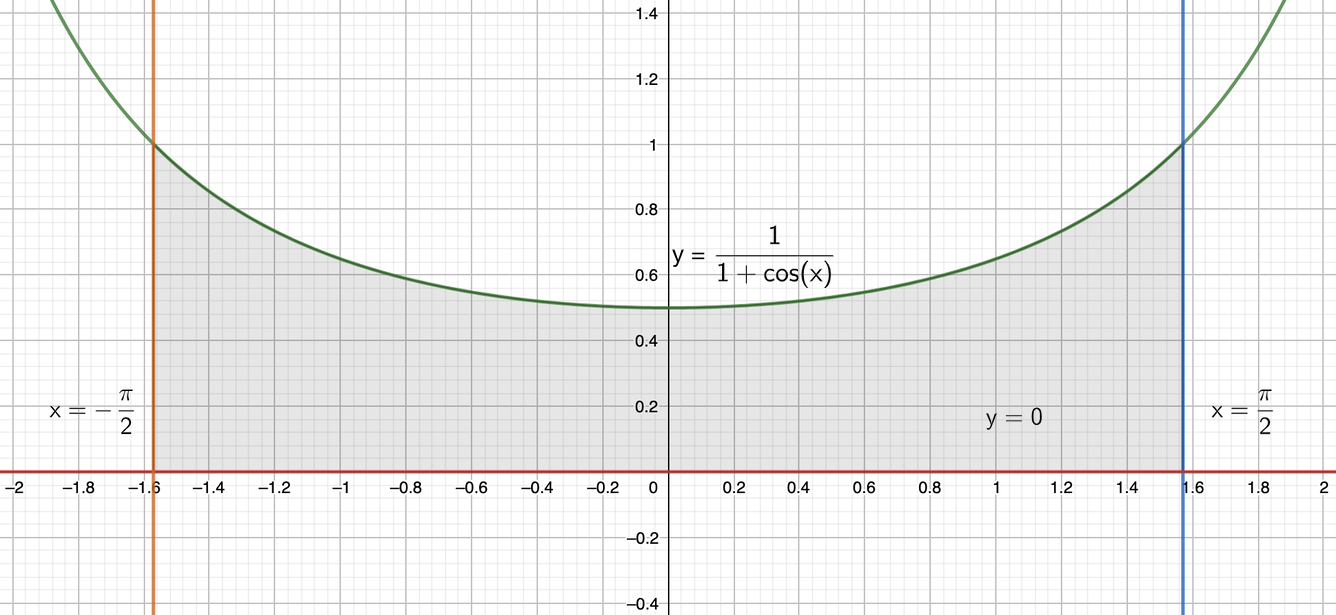
\includegraphics[width=300pt]{Figures/10.png}
\end{figure}

$=$\vspace{2.5mm}

/ Замена: $t= $  \hspace{2.5mm}  $t=$ \vspace{2.5mm}\\
$dt=$ \hspace{2.5mm} $dt=$ /\vspace{2.5mm}

$=$\vspace{2.5mm}

Ответ: $ $

\subsection*{Задание 11. Найдите длину кривой, заданной в декартовых координатах.}

$=$\vspace{2.5mm}

\begin{figure}[ht!]
\centering
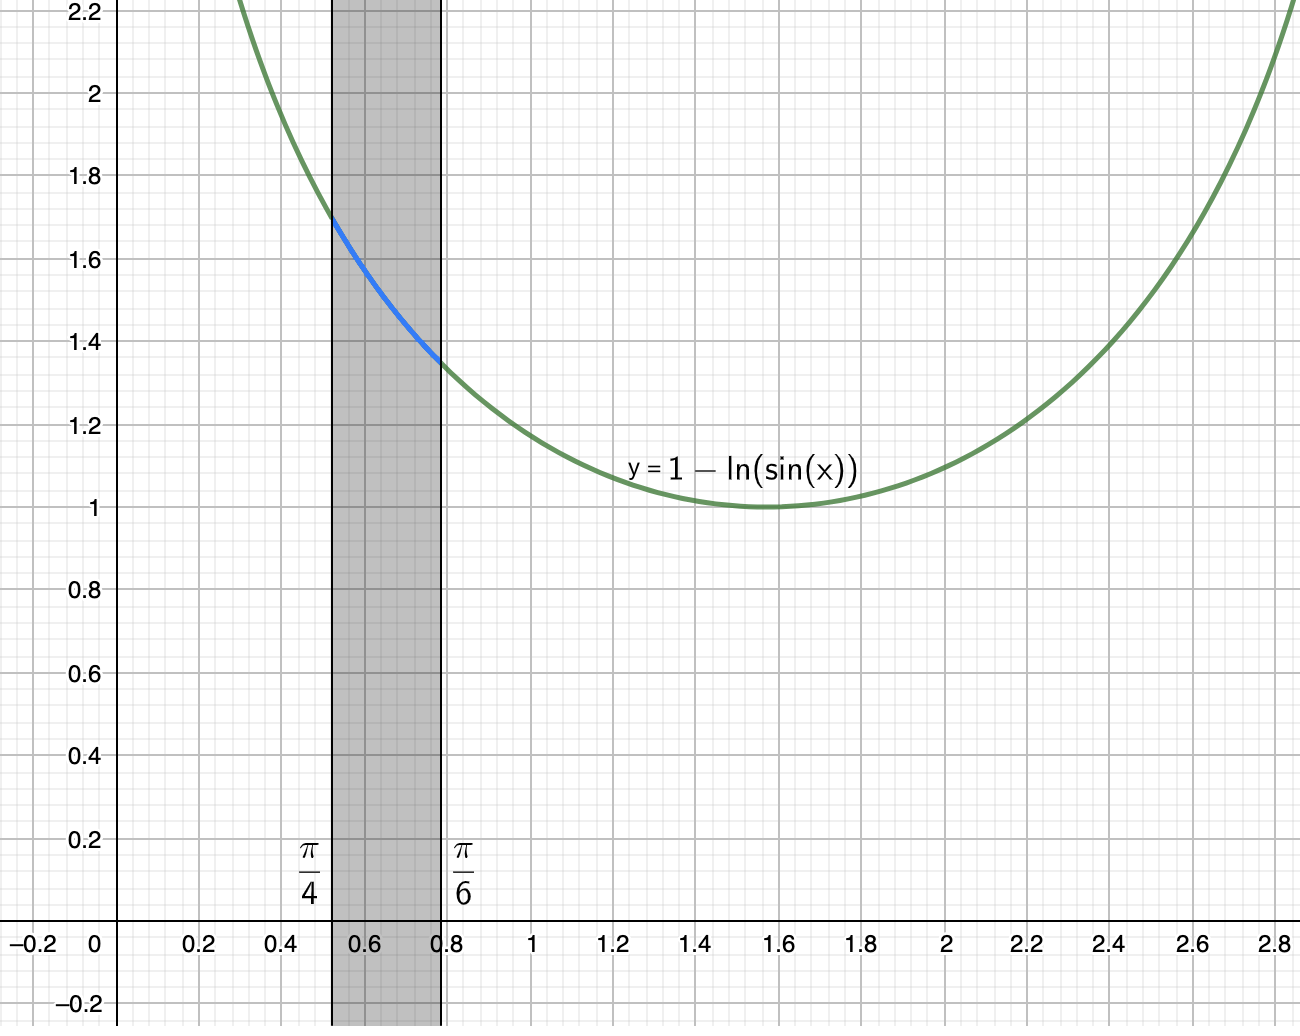
\includegraphics[width=325pt]{Figures/11.png}
\end{figure}

$L=$\vspace{2.5mm}

Ответ: $ $

\subsection*{Задание 12. Вычислите.}

а) Площадь, ограниченную осью абсцисс и верзиерой\vspace{2.5mm}\\
$\begin{cases}x=t\\
y=t\end{cases}$ \vspace{2.5mm}\\

\begin{figure}[ht!]
\centering
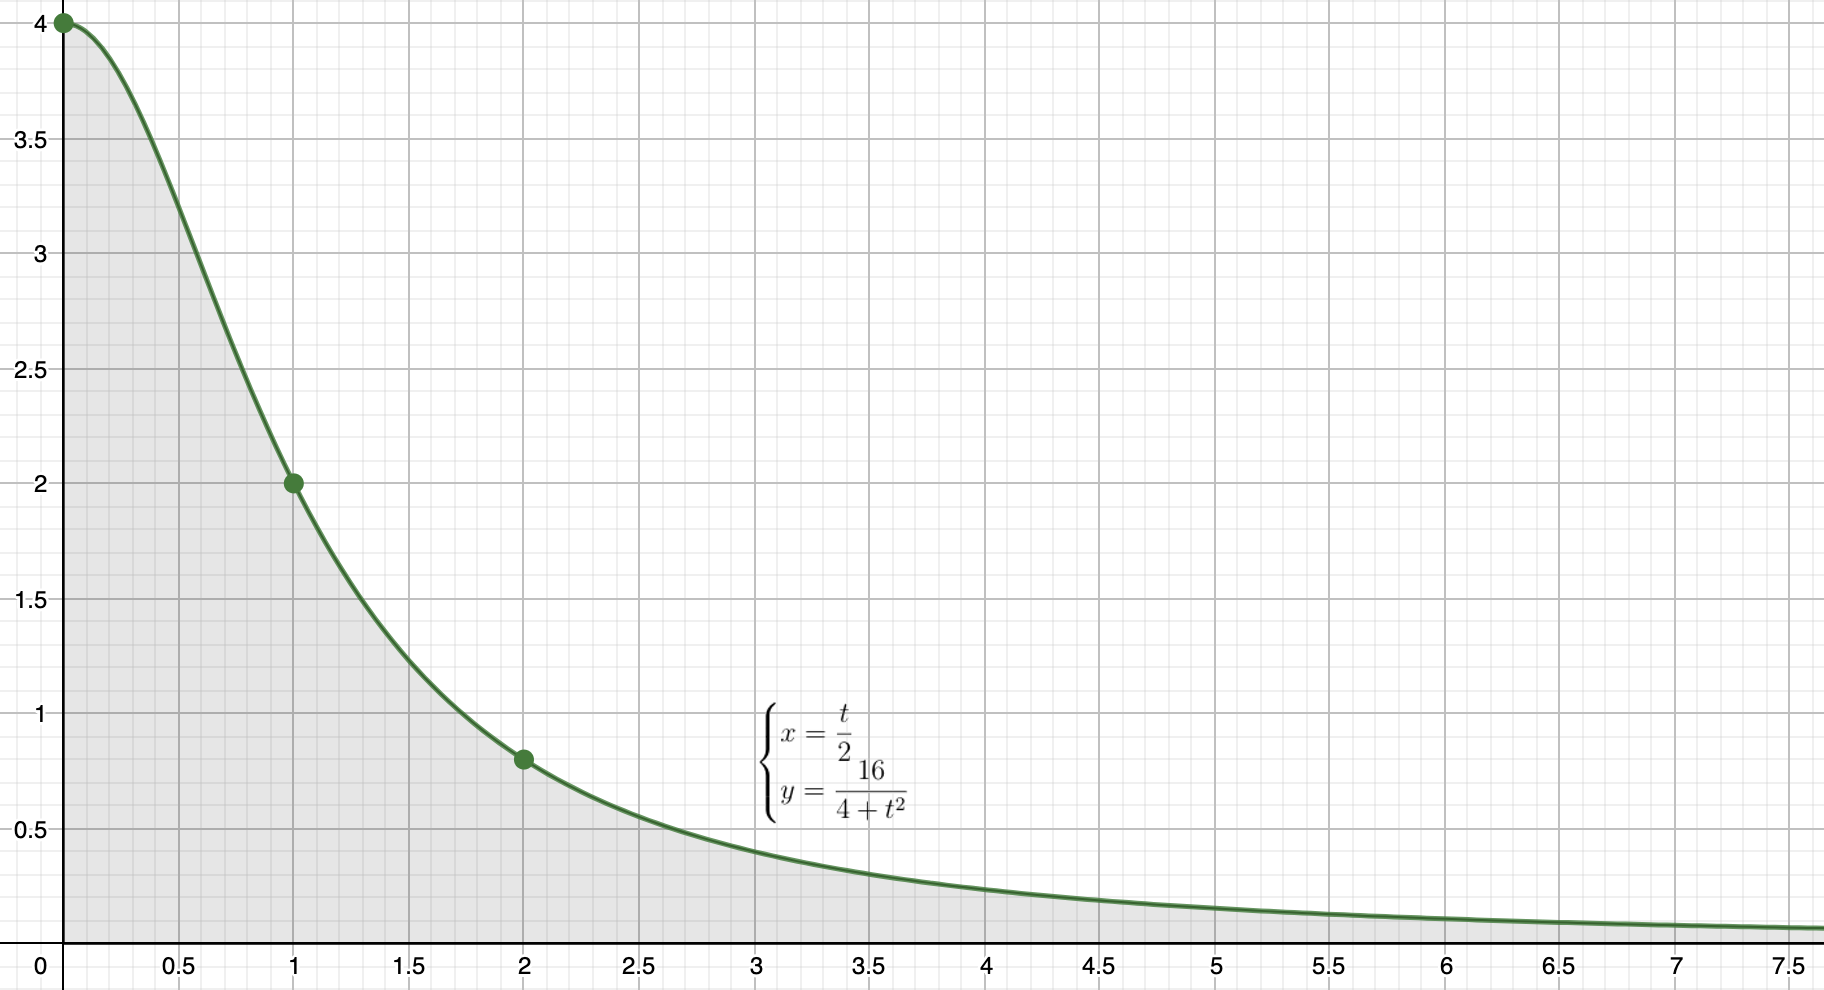
\includegraphics[width=325pt]{Figures/12a.png}
\end{figure}

$S=$\vspace{2.5mm}

/ Замена: $t= $  \hspace{2.5mm}  $t=$ \vspace{2.5mm}\\
$dt=$ \hspace{2.5mm} $dt=$ /\vspace{2.5mm}

$=$\vspace{2.5mm}

Ответ: $ $\vspace{2.5mm}

б) Длину дуги кривой\vspace{2.5mm}

$r=\varphi$\vspace{2.5mm}

\begin{figure}[ht!]
\centering
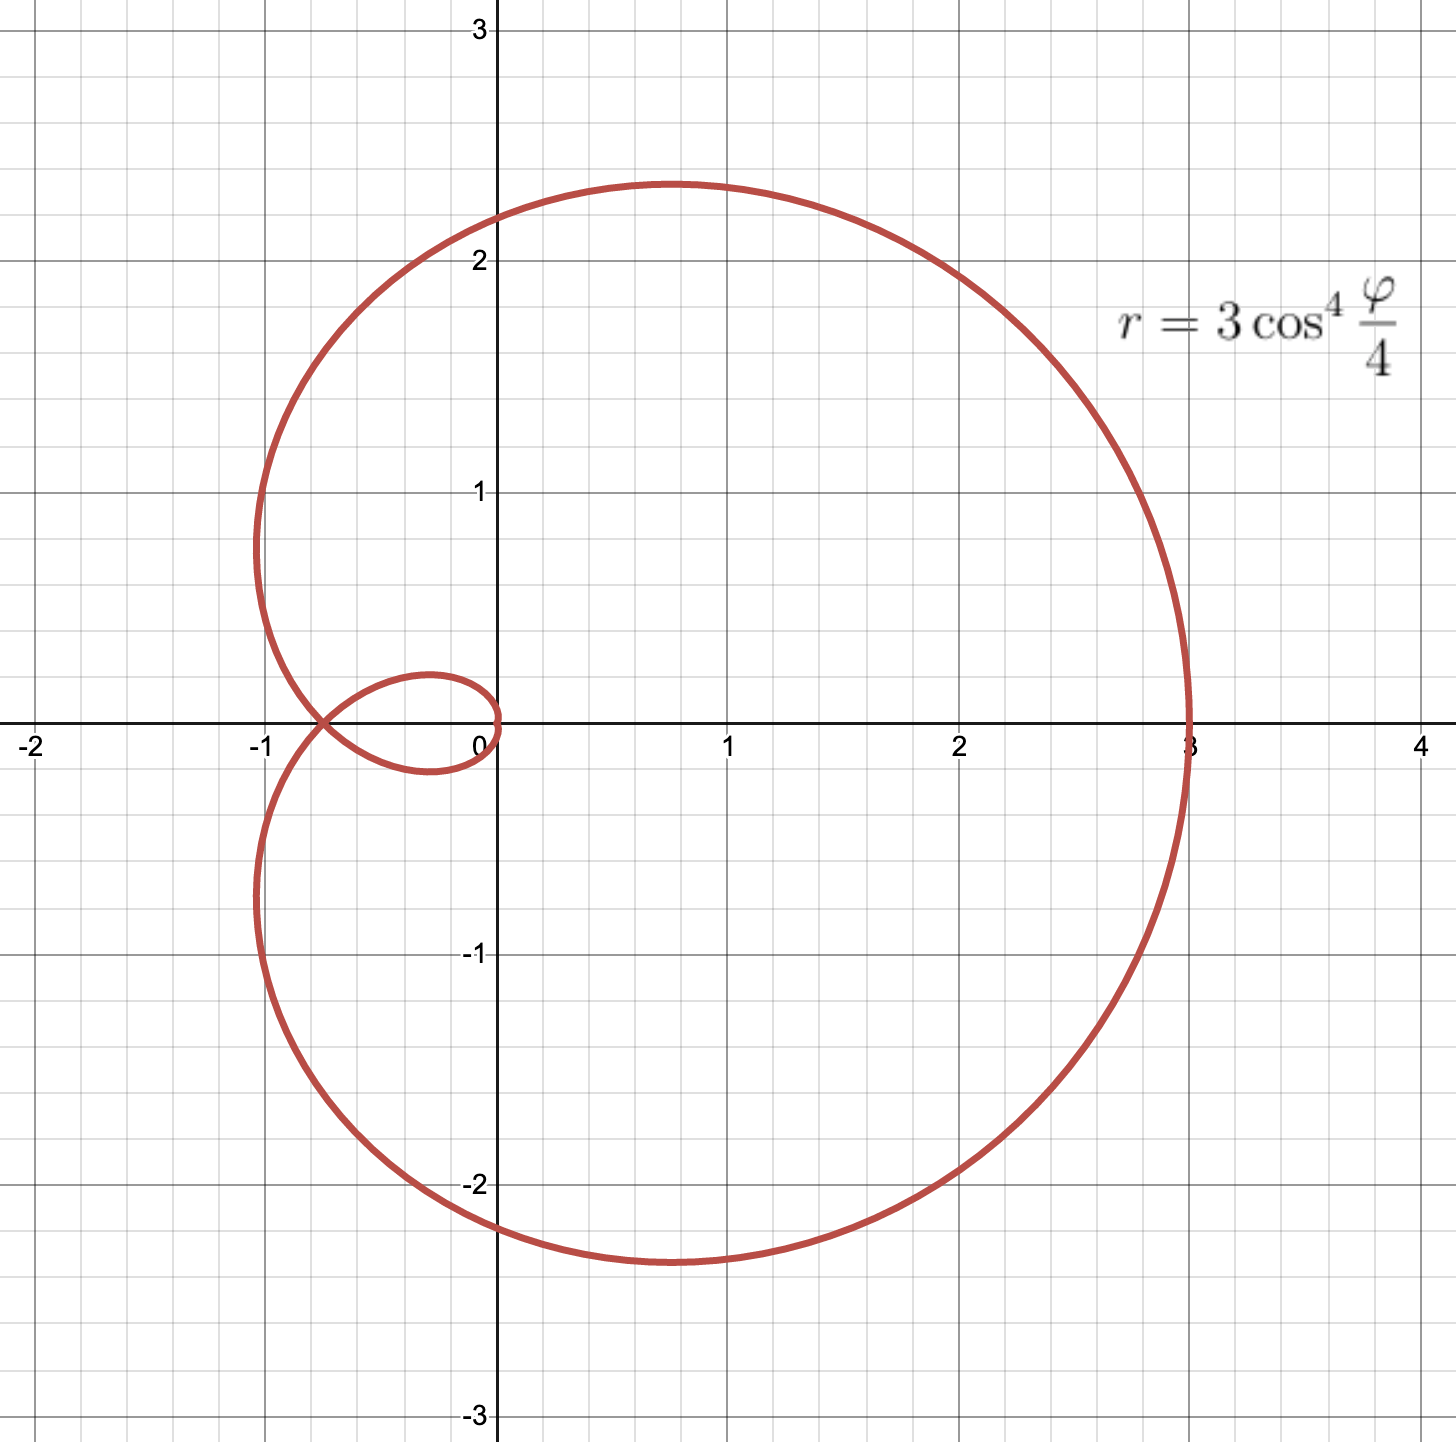
\includegraphics[width=225pt]{Figures/12b.png}
\end{figure}

$r\geq 0 \rightarrow \varphi \geq 0 $\vspace{2.5mm}

$L=$\vspace{2.5mm}

/ Замена: $t= $  \hspace{2.5mm}  $t=$ \vspace{2.5mm}\\
$dt=$ \hspace{2.5mm} $dt=$ /\vspace{2.5mm}

$=$\vspace{2.5mm}

Ответ: $ $

\subsection*{Задание 13. Найдите значение несобственного интеграла или\\установите его расходимость.}

а) $\int\limits^{+\infty }_{0}dx=\lim\limits _{b\to +\infty }\int\limits^{b}_{0}dx=$\vspace{2.5mm}

Ответ: $ $\vspace{2.5mm}

б) $\int\limits^{+\infty }_{0}dx=\lim\limits _{b\to +\infty }\int\limits^{b}_{0}dx=$\vspace{2.5mm}

Ответ: $ $

\end{document}